\documentclass[type=master]{thuthesis}
% 选项:
%   type=[bachelor|master|doctor|postdoctor], % 必选
%   secret,                                   % 可选
%   pifootnote,                               % 可选(建议打开)
%   openany|openright,                        % 可选,基本不用
%   arial,                                    % 可选,基本不用
%   arialtoc,                                 % 可选,基本不用
%   arialtitle                                % 可选,基本不用

% 所有其它可能用到的包都统一放到这里了,可以根据自己的实际添加或者删除。
\usepackage{thuthesis}
\usepackage{algorithm}
\usepackage{algorithmic}

\newcommand{\tbd}[1]{{\color{blue} #1}}
%\newtheorem{example}{例子}

% 定义所有的图片文件在 figures 子目录下
\graphicspath{{figures/}}

% 可以在这里修改配置文件中的定义。导言区可以使用中文。
% \def\myname{薛瑞尼}
\renewcommand{\algorithmicrequire}{ \textbf{输入:}} 

\begin{document}

%%% 封面部分
\frontmatter
\thusetup{
  %******************************
  % 注意:
  %   1. 配置里面不要出现空行
  %   2. 不需要的配置信息可以删除
  %******************************
  %
  %=====
  % 秘级
  %=====
  secretlevel={秘密},
  secretyear={10},
  %
  %=========
  % 中文信息
  %=========
  ctitle={线性规划问题中的信息获取},
  cdegree={本科},
  cdepartment={交叉信息研究院},
  cmajor={计算机科学与技术},
  cauthor={郑舒冉},
  csupervisor={李建教授},
  % 日期自动使用当前时间,若需指定按如下方式修改:
  % cdate={超新星纪元},
  %=========
  % 英文信息
  %=========
  etitle={Information Acquisition for Linear Optimization},
  % 这块比较复杂,需要分情况讨论:
  % 1. 学术型硕士
  %    edegree:必须为Master of Arts或Master of Science(注意大小写)
  %             “哲学、文学、历史学、法学、教育学、艺术学门类,公共管理学科
  %              填写Master of Arts,其它填写Master of Science”
  %    emajor:“获得一级学科授权的学科填写一级学科名称,其它填写二级学科名称”
  % 2. 专业型硕士
  %    edegree:“填写专业学位英文名称全称”
  %    emajor:“工程硕士填写工程领域,其它专业学位不填写此项”
  % 3. 学术型博士
  %    edegree:Doctor of Philosophy(注意大小写)
  %    emajor:“获得一级学科授权的学科填写一级学科名称,其它填写二级学科名称”
  % 4. 专业型博士
  %    edegree:“填写专业学位英文名称全称”
  %    emajor:不填写此项
  edegree={Bachelor of Engineering},
  emajor={Computer Science and Technology},
  eauthor={Shuran Zheng},
  esupervisor={Professor Jian Li},
  ckeywords={论文},
  ekeywords={thesis}
}

% 定义中英文摘要和关键字
\begin{cabstract}\end{cabstract}

% 如果习惯关键字跟在摘要文字后面,可以用直接命令来设置,如下:
% \ckeywords{\TeX, \LaTeX, CJK, 模板, 论文}

\begin{eabstract}
\end{eabstract}

% \ekeywords{\TeX, \LaTeX, CJK, template, thesis}

% 如果使用授权说明扫描页,将可选参数中指定为扫描得到的 PDF 文件名,例如:
% \makecover[scan-auth.pdf]
\makecover

%% 目录
\tableofcontents

%% 符号对照表
%\begin{denotation}[3cm]
\item[HPC] 高性能计算 (High Performance Computing)
\item[cluster] 集群
\item[Itanium] 安腾
\item[SMP] 对称多处理
\item[API] 应用程序编程接口
\item[PI] 聚酰亚胺
\item[MPI] 聚酰亚胺模型化合物,N-苯基邻苯酰亚胺
\item[PBI] 聚苯并咪唑
\item[MPBI] 聚苯并咪唑模型化合物,N-苯基苯并咪唑
\item[PY] 聚吡咙
\item[PMDA-BDA]	均苯四酸二酐与联苯四胺合成的聚吡咙薄膜
\item[$\Delta G$] 活化自由能 (Activation Free Energy)
\item[$\chi$] 传输系数 (Transmission Coefficient)
\item[$E$] 能量
\item[$m$] 质量
\item[$c$] 光速
\item[$P$] 概率
\item[$T$] 时间
\item[$v$] 速度
\item[劝学] 君子曰:学不可以已。青,取之于蓝,而青于蓝;冰,水为之,而寒于水。木
  直中绳。輮以为轮,其曲中规。虽有槁暴,不复挺者,輮使之然也。故木受绳则直,金就
  砺则利,君子博学而日参省乎己,则知明而行无过矣。吾尝终日而思矣,不如须臾之所学
  也;吾尝跂而望矣,不如登高之博见也。登高而招,臂非加长也,而见者远;顺风而呼,
  声非加疾也,而闻者彰。假舆马者,非利足也,而致千里;假舟楫者,非能水也,而绝江
  河,君子生非异也,善假于物也。积土成山,风雨兴焉;积水成渊,蛟龙生焉;积善成德,
  而神明自得,圣心备焉。故不积跬步,无以至千里;不积小流,无以成江海。骐骥一跃,
  不能十步;驽马十驾,功在不舍。锲而舍之,朽木不折;锲而不舍,金石可镂。蚓无爪牙
  之利,筋骨之强,上食埃土,下饮黄泉,用心一也。蟹六跪而二螯,非蛇鳝之穴无可寄托
  者,用心躁也。—— 荀况
\end{denotation}



%%% 正文部分
\mainmatter
\chapter{引言}

\chapter{背景知识}
\section{组合纯探索问题}
\begin{definition}[General Sampling问题]
假设有$n$个均值分别为$\mu_1, \dots, \mu_n$的单位方差高斯分布$\mathcal{D}_1, \dots, \mathcal{D}_n$,均值$\mu_1,\dots,\mu_n$在一开始是未知的。在每个时间$t$,我们可以选择一个分布$\mathcal{D}_i$,并获取它的一个样例。令$O_1,\dots, O_k$为$\mathbb{R}^n$上$k$个不相交的集合,我们想要找到一个算法,可以以$1-\delta$的概率找到$\mu = (\mu_1, \mu_2,\dots, \mu_n)$所在的集合$O_j$, $j$是$1$到$k$之间的某一个数,且该算法使用的样例总个数尽量的少。
\end{definition}

\section{Change of Distribution定理}

令算法$\mathcal{A}$为General Sampling问题的一个$\delta$-正确算法,定义$\Pr_{\mathcal{A}, \mathcal{I}}[\mathcal{E}]$为当算法$\mathcal{A}$的输入为$\mathcal{I}$时发生事件$\mathcal{E}$的概率,定义$\mathbb{E}_{\mathcal{A}, \mathcal{I}}[X]$为当算法$\mathcal{A}$的输入为$\mathcal{I}$时,随机变量$X$的期望值。
\begin{theorem}\label{ChangeDistr}
令算法$\mathcal{A}$为General Sampling问题的一个$\delta$-正确算法,令$\mathcal{I}_\mu$为$n$个分布的均值为$\mu_1,\dots, \mu_n$的一个General Sampling问题,令$\tau_i$为表示算法$\mathcal{A}$测量$\mu_i$的次数的随机变量,那么对于事件$\mathcal{E}$, 有
\[
\sum_{i=1}^n \mathbb{E}_{\mathcal{A}, \mathcal{I}_\mu}[\tau_i]\cdot (\frac{1}{2}(\mu_i - \mu'_i)^2) \ge d\left(\Pr_{\mathcal{A}, \mathcal{I}_\mu}[\mathcal{E}], \Pr_{\mathcal{A}, \mathcal{I}_{\mu'}}[\mathcal{E}]\right),
\]
其中,
\[
d(x,y) = x \ln (x/y)+ (1-x)\ln\left((1-x)/(1-y)\right).
\]
\end{theorem}
\section{椭球法}
在这一节中,我们介绍经典的解决凸规划问题的椭球法,考虑一个凸规划问题
\begin{align}
  \min & \ f(x) \tag{convex}\\
  s.t. & \ g_i(x) \le 0,  \forall 1\le i\le m. \notag
\end{align}
定义一个凸规划问题的分离函数(separation oracle)为
\begin{definition}\label{separation}
一个凸规划问题的分离函数$Separation(x)$返回$i$若$g_i(x)>0$; 返回"feasible"若不存在$i$使得$g_i(x)>0$.
\end{definition}
对于分离函数能在多项式时间内求解的凸规划问题,我们可以用椭球法求出最优解,

\tbd{give the description of ellipsoid method...}  
\chapter{问题描述}
\section{目标函数未知的线性规划问题}
假设我们手上有一个线性规划问题,
\begin{align*}
\max &\ \ c^T x, \\
\textrm{ s.t. }& \ \ Ax \le b.
\end{align*}
我们想要找到这个问题的最优解,但是不知道这个问题里的目标函数,即向量$c$。假设我们可以通过一些方法去测量向量$c$里的每一个参数$c_i$,但是测量值$\tilde{c_i}$可能会有随机误差,假设这个随机误差服从均值为$0$,方差为$\sigma_i^2$的正态分布,即测量值$\tilde{c_i}$服从均值为$c_i$,方差为$\sigma^2$的正态分布。我们的目标是找到一个算法,能够保证有很高的概率可以找到正确的最优值,且使用的测量次数尽量少。

在这片论文中,我们假设对所有的$i$都有$\sigma_i=1$。在本文介绍的所有结论中,方差$\sigma_i\neq 1$的情形都可以由$\sigma_i=1$的情形通过简单推导得到;或者也可以把多次测量值的平均值当作一次测量,这样就可以直接使用本文中的结论。

下面我们举几个具体的例子。
\begin{example}[最短路问题]
假设我们想要求在图$E=(U,V)$上节点$s$到节点$t$的最短路,我们不知道每条边的边权,但可以每次选一条边去测量。这个问题就可以被描述成如下目标函数未知的线性规划问题
\begin{align*}
\max &\ \ -\sum_{(u,v)\in E} w_{uv} x_{uv},\\
\textrm{ s.t. }& \ \ \sum_v x_{uv} - \sum_v x_{vu} = 0, \ \forall u,\\
& \ \ x_{uv}\ge 0, \forall u,v.
\end{align*}
其中$E$为边集,$w_{uv}$为边权。
\end{example}

\begin{example}[最大流问题]
假设我们想求在图$E=(U,V)$上从$s$到$t$的最大流,但是我们不知道每条边的流量上限,但可以每次选一条边去测量。这个问题就可以被描述成如下目标函数未知的线性规划问题
\begin{align*}
\max &\ \ -\sum_{(u,v)\in E} c_{uv}x_{uv}, \\
\textrm{ s.t. }& \ \  y_v + y_{sv} \ge 1, \ \ \forall v: (s,v)\in E,\\
& \ \ y_v -y_u +y_{uv} \ge 0, \ \ \forall(u,v)\in E, u\neq s, v\neq t,\\
& \ \ -y_u + y_{ut}\ge 0, \ \ \forall u: (u,t)\in E.
\end{align*}
其中$E$为边集,$c_{uv}$为边的流量上限。
\end{example}

\section{$\delta$-正确算法}
由于随机误差的存在,我们只能期望以高概率找到正确的线性规划最优解。
\begin{definition}[$\delta$-正确算法]
一个算法$\mathcal{A}$是$\delta$-正确算法,如果对于任意目标函数未知的线性规划问题,算法$\mathcal{A}$输出正确最优解$x^* = \max_{Ax\le b} c^T x$的概率至少为$1-\delta$.
\end{definition}

\tbd{give an example of $\delta$-correct algorithm?}
\chapter{采样复杂度下界}
\label{cha:lower}
在这章中,我们对问题的下界进行分析。
\section{基于单个实例的下界}
我们首先给出一个基于单个实例的采样复杂度下界。
 \begin{theorem}\label{inslow}
        令$\mathcal{I}$为一个目标函数未知的线性规划问题$\max_{\{x:Ax\le b\}} c^T x$. 任何 $\delta$-正确算法使用的测量次数的期望值都至少为$\Omega(Low(\mathcal{I}) \ln \delta^{-1})$,其中$Low(\mathcal{I})$等于
		\begin{align*}
         \min_\tau \quad & \sum_{i=1}^n \tau_i\\
        s.t.\quad & \sum_{i=1}^n \frac{(x_i^{(k)} -x_i^*)^2}{\tau_i} \le \left( c^T (x^* - x^{(k)}) \right)^2, \forall k\\
         &\tau_i\ge 0, \forall i
        \end{align*}
$x^*$是正确的最优解 $\arg \max_{\{x:Ax\le b\}} c^T x$, $x^{(1)},\dots, x^{(k)}$是所有的基本可行解,即可行域构成的凸包$\{x:Ax\le b\}$上的所有的顶点.
\end{theorem}
\begin{proof}
由于我们的问题是\cite{WJMZBMR}中定义的General Sampling问题的一个特例, \cite{WJMZBMR}中的instance lower bound对于我们的问题也是成立的. \cite{WJMZBMR}中$Low(\mathcal{I})$的定义如下,
 \begin{align}
        \label{LowGeneral} \min_\tau \quad & \sum_{i=1}^n \tau_i, \\
        s.t.\quad & \sum_{i=1}^n (\nu_i-\mu_i)^2 \tau_i \ge 1, \forall \nu \in Alt(O), \notag\\
         &\tau_i\ge 0, \forall i, \notag
 \end{align}
 其中$\mu_i$是General Sampling问题中每一个臂的均值, 在我们的问题中等同于目标函数中的未知数$c_i$. 在我们的问题中,集合$O$等同于所有满足下述条件的$n$维向量$c'$的集合:当限制条件为$Ax\le b$时,目标函数$c'$和$c$有着相同的最优解$x^*$。而集合$Alt(O)$的定义是$O$的补集, 也就是当限制条件为$Ax\le b$时,与$c$有着不同的最优解的向量$c'$的集合。 
 
由上面的定义可知,一个向量$c'$属于$O$,当且仅当在目标函数为$c'$时,可行域凸包上的顶点都没有$x^*$优,即
 \begin{align} 
\label{defO} O = \{ d| d^T (x^{(k)} - x^*) \le 0, \forall k\} 
 \end{align}
 故在我们的问题中$Low(\mathcal{I})$就等于
 \begin{align} 
   \tag{program1}      \min_\tau \quad & \sum_{i=1}^n \tau_i, \\
        s.t.\quad & \sum_{i=1}^n (d_i-c_i)^2 \tau_i \ge 1, \forall d \notin O, \notag\\
         &\tau_i\ge 0, \forall i, \notag
 \end{align}
 将式~(\ref{defO})的定义代入~(\ref{program1})中, 我们可以得到
 \begin{align}
     \tag{program2}    \min_\tau \quad & \sum_{i=1}^n \tau_i,\\
        s.t.\quad & \{ d | \sum_{i=1}^n (d_i-c_i)^2 \tau_i \le 1\} \subseteq \{ d| d^T (x^{(k)} - x^*) \le 0, \forall k\} \notag \\
         &\tau_i\ge 0, \forall i. \notag
 \end{align}
 注意到左侧集合$\{ d | \sum_{i=1}^n (d_i-c_i)^2 \tau_i \le 1\}$是右侧集合$\{ d| d^T (x^{(k)} - x^*) \le 0, \forall k\}$的子集当且仅当对于每一个$k$, 左侧集合中使得$d^T (x^{(k)} - x^*)$最大的$d$满足$d^T (x^{(k)} - x^*) \le 0$。
 
所以我们可以进一步将~(\ref{program2})表示为:
\begin{align}
\tag{program3} \min_\tau \quad & \sum_{i=1}^n \tau_i,\\
        s.t.\quad & \max_d \left\{ d^T (x^{(k)} - x^*) {\Large|} \sum_{i=1}^n (d_i-c_i)^2 \tau_i \le 1\right\}  \le 0, \forall k \notag \\
         &\tau_i\ge 0, \forall i. \notag
 \end{align}
通过一些简单的计算,可以求得上式左侧的最大值为$\max_d d^T (x^{(k)} - x^*) = (x^{(k)} - x^*)^T c + \sqrt{\sum_i (x^{(k)}_i - x^*_i)^2/\tau_i}$. 
所以~(\ref{program3})可以表示为
\begin{align*}
  \min_\tau \quad & \sum_{i=1}^n \tau_i,\\
        s.t.\quad & (x^{(k)} - x^*)^T c + \sqrt{\sum_i (x^{(k)}_i - x^*_i)^2/\tau_i}  \le 0, \forall k\\
         &\tau_i\ge 0, \forall i. 
 \end{align*}

稍加整理,我们就可以得到定理中的结果
\begin{align*}
         \min_\tau \quad & \sum_{i=1}^n \tau_i\\
        s.t.\quad & \sum_{i=1}^n \frac{(x_i^{(k)} -x_i^*)^2}{\tau_i} \le \left( c^T (x^* - x^{(k)}) \right)^2, \forall k\\
         &\tau_i\ge 0, \forall i
\end{align*}
\end{proof}

\section{基于最坏情形的下界}


    \begin{theorem}
        令$n$为一个正整数,$0<\delta<0.1$, 对于任何$\delta$-正确算法$\mathcal{A}$, 存在无限多个含$n$个变量的线性规划问题, $\mathcal{I}_1, \mathcal{I}_2, \dots$,使得$\mathcal{A}$在$\mathcal{I}_k$上使用的测量次数的期望为
        \[
        \Omega\left(Low(\mathcal{I}_k)(n+\ln \delta^{-1}) \right)
        \]
        且$Low(\mathcal{I}_k)$的极限趋于无穷大。
    \end{theorem}
 在证明中,我们利用下面引理构造出一个可行域$Ax\le b$,
 \begin{lemma}\label{mSets}
 令$n$为一个正整数,则存在$m=2^{cn}$个集合$S_1,\dots,S_m \subseteq [n]$使得$c$为一个常数,且对于所有的$i$,都有$\vert S_i \vert = l = \Omega(n)$, 对于所有$i\neq j$,都有$\vert S_i \cap S_j\vert \le l/2$.
 \end{lemma}
  \begin{proof}
  令每个$S_i$都为一个随机等概率选取的$[n]$的长度为$l$的子集,那么对于任意$i\neq j$,我们有
  \[
  \Pr[\vert S_i \cap S_j \vert > l/2]\le 2^{-\Omega(n)}.
  \]
  所以我们可以选取足够小的$c$使得
  \[
  \Pr[\exists i\neq j, \vert S_i \cap S_j \vert > l/2]\le m^2 2^{-\Omega(n)}< 1.
  \]
  \end{proof}
  
  下面我们给出定理中$\mathcal{I}_1, \mathcal{I}_2, \dots$的构造方法。
  我们先给出可行域$Ax\le b$的定义。给定变量个数$n$,令$S_1,\dots,S_m \subseteq [n]$为满足上述引理中条件的集合。对于一个集合$S\subseteq [n]$, 定义$n$维空间中的点$P_S$的第$j$维为$1$若$j\in S$, 否则为$0$。我们令可行域$Ax\le b$为$P_{S_1},\dots, P_{S_m}$和原点构成的凸包。
  
  我们再给出目标函数的构造。给定$\Delta \in (0, 0,1)$, 和集合$C\subseteq [n]$, 我们令线性规划问题$\mathcal{I}_{\Delta, C}$的目标函数$c^T x$满足:$c_i = \Delta$若$i\in C$,否则$c_i = - \Delta$。
  
  由上述定义可知$\mathcal{I}_{\Delta, S_i}$的最优解即为$P_{S_i}$。下面我们固定一个$\Delta\in (0,0,1)$和一个$\delta$-正确算法$\mathcal{A}$,并证明必定存在$S_k$,$1\le k \le m$使得$\mathcal{A}$在$\mathcal{I}_{\Delta, S_k}$上使用的测量次数的期望为$\Omega\left(Low(\mathcal{I}_{\Delta, S_k})(n+\ln \delta^{-1}) \right).$
        
 定义$\Pr[\mathcal{A}(\mathcal{I}_{\Delta, S_i}) = P_{S_j}]$为当线性规划问题是$\mathcal{I}_{\Delta, S_i}$时,算法$\mathcal{A}$输出的最优解为$P_{S_j}$的概率。那么应当有
 \[
 \Pr[\mathcal{A}(\mathcal{I}_{\Delta, S_i}) = P_{S_i}] \ge 1-\delta,
 \]
 和
 \[
 \sum_{j: j\neq i} \Pr[\mathcal{A}(\mathcal{I}_{\Delta, S_i}) = P_{S_j}] \le \delta.
 \]
 那么一定存在$S_k\neq S_i$,使得
 \[
	\Pr[\mathcal{A}(\mathcal{I}_{\Delta, S_i}) = P_{S_k}] \le 2\delta/m.
 \]
 结合$\Pr[\mathcal{A}(\mathcal{I}_{\Delta, S_k}) = P_{S_k}] \ge 1 - \delta> 0.9$ 和 定理\ref{ChangeDistr}, 令$T$为算法$\mathcal{A}$在输入为$\mathcal{I}_{\Delta,S_k}$时,使用的测量次数,我们有
 \begin{align*}
\mathbb{E}[T]\cdot (2 \Delta^2) &\ge d\left(\Pr[\mathcal{A}(\mathcal{I}_{\Delta, S_k}) = P_{S_k}],\Pr[\mathcal{A}(\mathcal{I}_{\Delta, S_i}) = P_{S_k}]\right) \\
&\ge \Omega(\ln(m/\delta)\\
& = \Omega(n + \ln(1/\delta)),
\end{align*}
这里我们用到了$d(1-\delta,\delta)$的性质: 对于$0<\delta<0.1$, 有$d(1-\delta,\delta)\ge 0.4 \ln(1/\delta)$。所以我们有$E[T]\ge \Omega\left(\Delta^{-2}(n + \ln(1/\delta))\right)$.

同时由引理\ref{mSets}中$S_1,\dots, S_m$的性质,我们可以证明令所有的$\tau_i = \frac{2}{l\Delta^2}$是$Low(\mathcal{I}_{\Delta, S_k})$中的一个可行解,故有$Low(\mathcal{I}_{\Delta, S_k})=\Theta(\frac{2n}{l\Delta^2}) = \Theta(\Delta^{-2})$. 
所以$\mathcal{A}$在$\mathcal{I}_{\Delta, S_k}$上使用的测量次数的期望为$\Omega\left(Low(\mathcal{I}_{\Delta, S_k})(n+\ln (\delta^{-1})) \right).$

取$\Delta = 1, 1/2, 1/3, \dots$,即可得定理中的结论。

\chapter{算法分析}
\label{cha:algo}
在这章中,我们给出一个可以与下界比较且较优的算法,并对正确性和采样复杂度进行分析。
\section{逐步排除算法}
  再给出算法之前,我们先定义一个函数$LowAll(S, \varepsilon, \delta)$,这里$S$是一个$n$维空间中的点集,$\varepsilon$和$\delta$是两个常数,这个函数的返回值是一个长度为$n$的向量,表示了我们至少需要测量每个$c_i$多少次, 才能以至少$1-\delta$的概率、$\varepsilon$的精度,估计$S$中任意一对点之间的目标函数值的差. 定义函数$LowAll(S, \varepsilon, \delta)$为:
        \begin{align*}
        \min_{\tau} \quad & \sum_{i=1}^n \tau_i\\
        s.t.\quad & \sum_{i=1}^n \frac{(x_i -y_i)^2}{\tau_i} \le \frac{\varepsilon^2}{2 \ln(2/\delta)}, \forall x, y \in S\\
         &\tau_i\ge 0, \forall i.
        \end{align*}
我们的逐步排除算法在一开始将所有可能的最优解(即可行域的所有顶点)纳入考虑范围,每一次循环中算法都会根据$LowAll(S, \varepsilon, \delta)$的值对每个$c_i$进行测量,再根据测量结果删除掉与最优解的差大于某一个值的点,每一次循环中算法都会将精度$\varepsilon$减半,从而能够排除掉更多的点。当只剩下一个未被排除的点时,算法结束。
	\begin{algorithm}[H]                      % enter the algorithm environment
                \caption{逐步排除算法}
                \label{Algo1}
                \begin{algorithmic}[1]
                	\REQUIRE 线性规划问题$\mathcal{I} = \max_{Ax\le b} c^T x$.
                    \STATE $S^1\gets$所有基本可行解的集合,或者说可行域$\{x: Ax\le b\}$所有顶点的集合
                    \STATE $r\gets 1$
                    \STATE $\lambda\gets 10$
                    \WHILE{$|S^r|>1$}
                        \STATE $\varepsilon^r \gets 2^{-r}$, $\delta^r \gets \delta/(10 r^2 |S^1|^2)$
                        \STATE $(m^r_1, \dots, m^r_n) \gets LowAll(S^r, \varepsilon^r/\lambda, \delta^r)$
                        \STATE 对$c_i$进行$m^r_i$次测量, 令$\hat{c}^r_i$为这$m^r_i$次测量的均值
                        \STATE 令$x^r$为当目标函数是$\hat{c}^r$时,集合$S^r$中的最优值,即
                        $x^r = \arg \max_{x\in S^r} x^T \hat{c}^r$.
                        \STATE 去除$S^r$中我们认为在目标函数为$\hat{c}^r$时,比$x^r$要差至少$\varepsilon^r/2+2\varepsilon^r/\lambda$的点,即$S^{r+1} \gets \{ x\in S^r: x^T \hat{c}^r \ge (x^r)^T \hat{c}^r-\varepsilon^r/2-2\varepsilon^r/\lambda\}$
                        \STATE $r \gets r+1$
                    \ENDWHILE
                    \STATE 输出$S^r$中仅剩的一个点。
                \end{algorithmic}
                \end{algorithm}

    \begin{theorem}
    令$\mathcal{I}$为一个目标函数未知的线性规划问题$\max_{\{x:Ax\le b\}} c^T x$. 有至少$1-\delta$的概率, 逐步排除算法会输出正确的最优解, 且使用的测量次数为
     \[
        O\left( Low(\mathcal{I}) \ln \Delta^{-1} ( n + \ln \delta^{-1} + \ln \ln \Delta^{-1})\right),
     \]
     其中$n$是线性规划变量的个数, $\Delta$是目标函数为$c$时,最优的基本可行解与次优的基本可行解之间的差值,即
     \[
     \Delta = \max_{x\in S^1} c^T x - \max_{x\in S^1 - x^*} c^T x.
     \]
    \end{theorem}
	
\section{算法正确性}
 在这一节中,我们证明该算法是$\delta$-正确算法。在证明中我们会用到下面这个引理,
    \begin{lemma}\label{lem1}
 考虑目标函数$c = (c_1, \dots, c_n)$, 假设我们对$c_i$进行$\tau_i$次测量,每一次测量的误差服从标准高斯分布,令$X_i$为这$\tau_i$次测量的平均值。那么对任意$n$维向量$p$, 有 
    \[
    \Pr\left[ |p^T X - p^T c|\ge \varepsilon\right] \le 2 \exp\{-\frac{\varepsilon^2}{2 \sum p_i^2/\tau_i}\}
    \]
    \end{lemma}
    \begin{proof}
    由定义可知, $p^T X - p^T c$服从均值为$0$方差为$\sum_i p_i^2/\tau_i$的高斯分布,由高斯分布的tail bound即可得到上述不等式. 
    \end{proof}
定义事件$\mathcal{E}$为下述条件成立的事件$$|(x-y)^T (\hat{c}^r - c))|\le \varepsilon^r /\lambda,\ \forall r, \forall x,y \in S^r.$$ 
根据引理~\ref{lem1}和union bound, $\Pr[\mathcal{E}]\ge 1-\delta$. \tbd{prove this?} 那么我们只需证明以下引理,
\begin{lemma}\label{correct}
在事件$\mathcal{E}$成立的时候,最优解$x^* = \max_{Ax\le b} c^T x$不会被算法删除。
\end{lemma}
\begin{proof}
假设$x^*$在第$r$个循环中被删除,即$x^* \in S^r$, $x^* \notin S^{r+1}$,那么我们有
\[
\langle \hat{c}^r, x^*\rangle < \langle \hat{c}^r, x^r\rangle-\varepsilon^r/2-2\varepsilon^r/\lambda.
\]
即
\[
\langle \hat{c}^r, x^* - x^r\rangle < -\varepsilon^r/2-2\varepsilon^r/\lambda.
\]
而由$x^*$的定义知
\[
\langle c, x^* - x^r\rangle > 0.
\]
结合两个不等式,我们可以得到
\[
\langle c - \hat{c}^r, x^* - x^r\rangle > \varepsilon^r/2 + 2\varepsilon^r/\lambda > \varepsilon^r /\lambda,
\]
由于$x^*$和$x^r$都是$S^r$中元素,这与$\mathcal{E}$成立矛盾。故当$\mathcal{E}$成立,最优解$x^*$不会被算法删除。
\end{proof}
\section{采样复杂度分析}

我们再对算法的采样复杂度进行分析。与上一节中一样,定义事件$\mathcal{E}$为下述条件成立的事件$$|(x-y)^T (\hat{c}^r - c))|\le \varepsilon^r /\lambda,\ \forall r, \forall x,y \in S^r.$$ 
根据引理~\ref{lem1}和union bound, $\Pr[\mathcal{E}]\ge 1-\delta$。

我们首先给出算法循环次数的上界,
\begin{lemma}\label{itrnum}
当$\mathcal{E}$成立时,算法循环次数不会超过$\lfloor \log(\Delta^{-1})\rfloor + 1$,其中$\Delta$是当目标函数为$c$时,最优的基本可行解与次优的基本可行解之间的差值,即
     \[
     \Delta = \max_{x\in S^1} c^T x - \max_{x\in S^1 - x^*} c^T x.
     \]
\end{lemma}
\begin{proof}
我们只需证明在第$r$次循环结束后,$S^{r+1}$中所有的元素$s$都满足以下条件,
\[
\langle c, x^* - s\rangle < \varepsilon^r, \ \forall s\in S^{r+1}.
\]
假设在进入第$r$次循环时,存在$s\in S^r$使得
\[
\langle c, x^* - s\rangle > \varepsilon^r,
\]
那么由于$\mathcal{E}$成立,且我们选择$\lambda=10$,
\[
\langle c^r, x^* - s\rangle > \langle c, x^* - s\rangle - \varepsilon^r/\lambda > (1-1/\lambda)\varepsilon^r  >\varepsilon^r/2 + 2\varepsilon^r/\lambda,
\]
又因为引理\ref{correct},$x^*$一定存在于$S^r$中。故$s$会在第$r$个循环中被删除。
\end{proof}
下面我们给出算法在第$r$次循环中使用的测量次数的上界。令$n$维向量$\tau$为定理\ref{inslow}中定义的$Low(\mathcal{I})$的返回值. 考虑第$r$次循环, 定义$$\alpha = 32 \lambda^2 \ln(2/\delta^r).$$ 我们证明$m = \alpha \tau^*$满足$LowAll(S^r, \varepsilon^r, \delta^r)$所有的约束条件. 对于任意的$x,y\in S^r$, 我们有 
\begin{align*}
\sum \frac{(x_i-y_i)^2}{m_i} &= \frac{1}{\alpha} \sum \frac{(x_i-y_i)^2}{\tau_i^*}\\
& = \frac{1}{\alpha} \sum \frac{(x_i-x^*_i + x^*_i - y_i)^2}{\tau_i^*}\\
& \le \frac{1}{\alpha} \sum \frac{2(x_i-x^*_i)^2 + 2(x^*_i - y_i)^2}{\tau_i^*}\\
& \le \frac{2}{\alpha} \left((c^T(x^*-x))^2 + (c^T(x^* - y))^2\right)\\
& \le \frac{4}{\alpha} (\varepsilon^{r-1})^2 = \frac{(\varepsilon^r)^2}{2\lambda^2 \ln(2/\delta^r)}.
\end{align*}
在第四行中,我们用到了$Low$函数\ref{LowGeneral}的定义,在第五行中我们用到了引理\ref{itrnum}证明中的结论。

所以在第$r$次循环中,我们使用的测量次数不会超过
\[
\sum_i m_i = \alpha \sum_i \tau_i^* = O(Low(\mathcal{I})(\ln r + \ln |S^r| + \ln \delta^{-1}).
\]
结合引理\ref{itrnum},循环次数不会超过$\lfloor \log(\Delta^{-1})\rfloor + 1$,故算法使用的总测量数不会超过
\[
O\left( Low(\mathcal{I}) \ln \Delta^{-1} ( n + \ln \delta^{-1} + \ln \ln \Delta^{-1})\right).
\]

%\chapter{算法实现}
注意到在上一章介绍的逐步迭代算法中,函数$LowAll(S, \varepsilon, \delta)=$
\begin{align}
   \tag{lowall}    \min_{\tau} \quad & \sum_{i=1}^n \tau_i\\
        s.t.\quad & \sum_{i=1}^n \frac{(x_i -y_i)^2}{\tau_i} \le \frac{\varepsilon^2}{2 \ln(2/\delta)}, \forall x, y \in S\\
         &\tau_i\ge 0, \forall i.
\end{align}
中的目标函数和限制条件都是凸函数,所以该函数可以用凸规划算法进行求解,如次梯度法、内点法、椭球法等\cite{}。但是注意到该函数限制条件个数是指数级别的,直接套用凸规划算法会非常低效。在这一章中,我们给出一个基于二次规划算法的实现方法。

考虑使用椭球法来求解$LowAll(S, \varepsilon, \delta)$,我们只需考虑如何实现分离函数~(\ref{separation}),即
\begin{definition}
$LowAll(S, \varepsilon, \delta)$的分离函数$Separation(\tau)$返回$x,y\in S$若$\sum_{i=1}^n \frac{(x_i -y_i)^2}{\tau_i} > \frac{\varepsilon^2}{2 \ln(2/\delta)}$; 返回"feasible"若不存在$x,y\in S$使得$\sum_{i=1}^n \frac{(x_i -y_i)^2}{\tau_i} > \frac{\varepsilon^2}{2 \ln(2/\delta)}$。
\end{definition}




%%% 其它部分
\backmatter

%% 本科生要这几个索引,研究生不要。选择性留下。
% 插图索引
\listoffigures
% 表格索引
\listoftables
% 公式索引
\listofequations


%% 参考文献
% 注意:至少需要引用一篇参考文献,否则下面两行可能引起编译错误。
% 如果不需要参考文献,请将下面两行删除或注释掉。
\bibliographystyle{thuthesis-numerical}
\bibliography{ref/refs}


%% 致谢
% 如果使用声明扫描页,将可选参数指定为扫描后的 PDF 文件名,例如:
% \begin{acknowledgement}[scan-statement.pdf]
\begin{acknowledgement}
  感谢导师李建教授在整个毕业设计中对我的耐心指导,他的言传身教将使
  我终生受益。同时也感谢陈立杰同学对我的帮助。

  感谢 \thuthesis,它的存在让我的论文写作轻松自在了许多,让我的论文格式规整漂亮了
  许多。
\end{acknowledgement}


%% 附录
%\begin{appendix}
%\chapter{外文资料原文}
\label{cha:engorg}

\title{The title of the English paper}

\textbf{Abstract:} As one of the most widely used techniques in operations
research, \emph{ mathematical programming} is defined as a means of maximizing a
quantity known as \emph{bjective function}, subject to a set of constraints
represented by equations and inequalities. Some known subtopics of mathematical
programming are linear programming, nonlinear programming, multiobjective
programming, goal programming, dynamic programming, and multilevel
programming$^{[1]}$.

It is impossible to cover in a single chapter every concept of mathematical
programming. This chapter introduces only the basic concepts and techniques of
mathematical programming such that readers gain an understanding of them
throughout the book$^{[2,3]}$.


\section{Single-Objective Programming}
The general form of single-objective programming (SOP) is written
as follows,
\begin{equation}\tag*{(123)} % 如果附录中的公式不想让它出现在公式索引中,那就请
                             % 用 \tag*{xxxx}
\left\{\begin{array}{l}
\max \,\,f(x)\\[0.1 cm]
\mbox{subject to:} \\ [0.1 cm]
\qquad g_j(x)\le 0,\quad j=1,2,\cdots,p
\end{array}\right.
\end{equation}
which maximizes a real-valued function $f$ of
$x=(x_1,x_2,\cdots,x_n)$ subject to a set of constraints.

\newtheorem{mpdef}{Definition}[chapter]
\begin{mpdef}
In SOP, we call $x$ a decision vector, and
$x_1,x_2,\cdots,x_n$ decision variables. The function
$f$ is called the objective function. The set
\begin{equation}\tag*{(456)} % 这里同理,其它不再一一指定。
S=\left\{x\in\Re^n\bigm|g_j(x)\le 0,\,j=1,2,\cdots,p\right\}
\end{equation}
is called the feasible set. An element $x$ in $S$ is called a
feasible solution.
\end{mpdef}

\newtheorem{mpdefop}[mpdef]{Definition}
\begin{mpdefop}
A feasible solution $x^*$ is called the optimal
solution of SOP if and only if
\begin{equation}
f(x^*)\ge f(x)
\end{equation}
for any feasible solution $x$.
\end{mpdefop}

One of the outstanding contributions to mathematical programming was known as
the Kuhn-Tucker conditions\ref{eq:ktc}. In order to introduce them, let us give
some definitions. An inequality constraint $g_j(x)\le 0$ is said to be active at
a point $x^*$ if $g_j(x^*)=0$. A point $x^*$ satisfying $g_j(x^*)\le 0$ is said
to be regular if the gradient vectors $\nabla g_j(x)$ of all active constraints
are linearly independent.

Let $x^*$ be a regular point of the constraints of SOP and assume that all the
functions $f(x)$ and $g_j(x),j=1,2,\cdots,p$ are differentiable. If $x^*$ is a
local optimal solution, then there exist Lagrange multipliers
$\lambda_j,j=1,2,\cdots,p$ such that the following Kuhn-Tucker conditions hold,
\begin{equation}
\label{eq:ktc}
\left\{\begin{array}{l}
    \nabla f(x^*)-\sum\limits_{j=1}^p\lambda_j\nabla g_j(x^*)=0\\[0.3cm]
    \lambda_jg_j(x^*)=0,\quad j=1,2,\cdots,p\\[0.2cm]
    \lambda_j\ge 0,\quad j=1,2,\cdots,p.
\end{array}\right.
\end{equation}
If all the functions $f(x)$ and $g_j(x),j=1,2,\cdots,p$ are convex and
differentiable, and the point $x^*$ satisfies the Kuhn-Tucker conditions
(\ref{eq:ktc}), then it has been proved that the point $x^*$ is a global optimal
solution of SOP.

\subsection{Linear Programming}
\label{sec:lp}

If the functions $f(x),g_j(x),j=1,2,\cdots,p$ are all linear, then SOP is called
a {\em linear programming}.

The feasible set of linear is always convex. A point $x$ is called an extreme
point of convex set $S$ if $x\in S$ and $x$ cannot be expressed as a convex
combination of two points in $S$. It has been shown that the optimal solution to
linear programming corresponds to an extreme point of its feasible set provided
that the feasible set $S$ is bounded. This fact is the basis of the {\em simplex
  algorithm} which was developed by Dantzig as a very efficient method for
solving linear programming.
\begin{table}[ht]
\centering
  \centering
  \caption*{Table~1\hskip1em This is an example for manually numbered table, which
    would not appear in the list of tables}
  \label{tab:badtabular2}
  \begin{tabular}[c]{|m{1.5cm}|c|c|c|c|c|c|}\hline
    \multicolumn{2}{|c|}{Network Topology} & \# of nodes &
    \multicolumn{3}{c|}{\# of clients} & Server \\\hline
    GT-ITM & Waxman Transit-Stub & 600 &
    \multirow{2}{2em}{2\%}&
    \multirow{2}{2em}{10\%}&
    \multirow{2}{2em}{50\%}&
    \multirow{2}{1.2in}{Max. Connectivity}\\\cline{1-3}
    \multicolumn{2}{|c|}{Inet-2.1} & 6000 & & & &\\\hline
    \multirow{2}{1.5cm}{Xue} & Rui  & Ni &\multicolumn{4}{c|}{\multirow{2}*{\thuthesis}}\\\cline{2-3}
    & \multicolumn{2}{c|}{ABCDEF} &\multicolumn{4}{c|}{} \\\hline
\end{tabular}
\end{table}

Roughly speaking, the simplex algorithm examines only the extreme points of the
feasible set, rather than all feasible points. At first, the simplex algorithm
selects an extreme point as the initial point. The successive extreme point is
selected so as to improve the objective function value. The procedure is
repeated until no improvement in objective function value can be made. The last
extreme point is the optimal solution.

\subsection{Nonlinear Programming}

If at least one of the functions $f(x),g_j(x),j=1,2,\cdots,p$ is nonlinear, then
SOP is called a {\em nonlinear programming}.

A large number of classical optimization methods have been developed to treat
special-structural nonlinear programming based on the mathematical theory
concerned with analyzing the structure of problems.
\begin{figure}[h]
  \centering
  
\includegraphics{thu-lib-logo}
  \caption*{Figure~1\quad This is an example for manually numbered figure,
    which would not appear in the list of figures}
  \label{tab:badfigure2}
\end{figure}

Now we consider a nonlinear programming which is confronted solely with
maximizing a real-valued function with domain $\Re^n$.  Whether derivatives are
available or not, the usual strategy is first to select a point in $\Re^n$ which
is thought to be the most likely place where the maximum exists. If there is no
information available on which to base such a selection, a point is chosen at
random. From this first point an attempt is made to construct a sequence of
points, each of which yields an improved objective function value over its
predecessor. The next point to be added to the sequence is chosen by analyzing
the behavior of the function at the previous points. This construction continues
until some termination criterion is met. Methods based upon this strategy are
called {\em ascent methods}, which can be classified as {\em direct methods},
{\em gradient methods}, and {\em Hessian methods} according to the information
about the behavior of objective function $f$. Direct methods require only that
the function can be evaluated at each point. Gradient methods require the
evaluation of first derivatives of $f$. Hessian methods require the evaluation
of second derivatives. In fact, there is no superior method for all
problems. The efficiency of a method is very much dependent upon the objective
function.

\subsection{Integer Programming}

{\em Integer programming} is a special mathematical programming in which all of
the variables are assumed to be only integer values. When there are not only
integer variables but also conventional continuous variables, we call it {\em
  mixed integer programming}. If all the variables are assumed either 0 or 1,
then the problem is termed a {\em zero-one programming}. Although integer
programming can be solved by an {\em exhaustive enumeration} theoretically, it
is impractical to solve realistically sized integer programming problems. The
most successful algorithm so far found to solve integer programming is called
the {\em branch-and-bound enumeration} developed by Balas (1965) and Dakin
(1965). The other technique to integer programming is the {\em cutting plane
  method} developed by Gomory (1959).

\hfill\textit{Uncertain Programming\/}\quad(\textsl{BaoDing Liu, 2006.2})

\section*{References}
\noindent{\itshape NOTE: These references are only for demonstration. They are
  not real citations in the original text.}

\begin{translationbib}
\item Donald E. Knuth. The \TeX book. Addison-Wesley, 1984. ISBN: 0-201-13448-9
\item Paul W. Abrahams, Karl Berry and Kathryn A. Hargreaves. \TeX\ for the
  Impatient. Addison-Wesley, 1990. ISBN: 0-201-51375-7
\item David Salomon. The advanced \TeX book.  New York : Springer, 1995. ISBN:0-387-94556-3
\end{translationbib}

\chapter{外文资料的调研阅读报告或书面翻译}

\title{英文资料的中文标题}

{\heiti 摘要:} 本章为外文资料翻译内容。如果有摘要可以直接写上来,这部分好像没有
明确的规定。

\section{单目标规划}
北冥有鱼,其名为鲲。鲲之大,不知其几千里也。化而为鸟,其名为鹏。鹏之背,不知其几
千里也。怒而飞,其翼若垂天之云。是鸟也,海运则将徙于南冥。南冥者,天池也。
\begin{equation}\tag*{(123)}
 p(y|\mathbf{x}) = \frac{p(\mathbf{x},y)}{p(\mathbf{x})}=
\frac{p(\mathbf{x}|y)p(y)}{p(\mathbf{x})}
\end{equation}

吾生也有涯,而知也无涯。以有涯随无涯,殆已!已而为知者,殆而已矣!为善无近名,为
恶无近刑,缘督以为经,可以保身,可以全生,可以养亲,可以尽年。

\subsection{线性规划}
庖丁为文惠君解牛,手之所触,肩之所倚,足之所履,膝之所倚,砉然响然,奏刀騞然,莫
不中音,合于桑林之舞,乃中经首之会。
\begin{table}[ht]
\centering
  \centering
  \caption*{表~1\hskip1em 这是手动编号但不出现在索引中的一个表格例子}
  \label{tab:badtabular3}
  \begin{tabular}[c]{|m{1.5cm}|c|c|c|c|c|c|}\hline
    \multicolumn{2}{|c|}{Network Topology} & \# of nodes &
    \multicolumn{3}{c|}{\# of clients} & Server \\\hline
    GT-ITM & Waxman Transit-Stub & 600 &
    \multirow{2}{2em}{2\%}&
    \multirow{2}{2em}{10\%}&
    \multirow{2}{2em}{50\%}&
    \multirow{2}{1.2in}{Max. Connectivity}\\\cline{1-3}
    \multicolumn{2}{|c|}{Inet-2.1} & 6000 & & & &\\\hline
    \multirow{2}{1.5cm}{Xue} & Rui  & Ni &\multicolumn{4}{c|}{\multirow{2}*{\thuthesis}}\\\cline{2-3}
    & \multicolumn{2}{c|}{ABCDEF} &\multicolumn{4}{c|}{} \\\hline
\end{tabular}
\end{table}

文惠君曰:“嘻,善哉!技盖至此乎?”庖丁释刀对曰:“臣之所好者道也,进乎技矣。始臣之
解牛之时,所见无非全牛者;三年之后,未尝见全牛也;方今之时,臣以神遇而不以目视,
官知止而神欲行。依乎天理,批大郤,导大窾,因其固然。技经肯綮之未尝,而况大坬乎!
良庖岁更刀,割也;族庖月更刀,折也;今臣之刀十九年矣,所解数千牛矣,而刀刃若新发
于硎。彼节者有间而刀刃者无厚,以无厚入有间,恢恢乎其于游刃必有余地矣。是以十九年
而刀刃若新发于硎。虽然,每至于族,吾见其难为,怵然为戒,视为止,行为迟,动刀甚微,
謋然已解,如土委地。提刀而立,为之而四顾,为之踌躇满志,善刀而藏之。”

文惠君曰:“善哉!吾闻庖丁之言,得养生焉。”


\subsection{非线性规划}
孔子与柳下季为友,柳下季之弟名曰盗跖。盗跖从卒九千人,横行天下,侵暴诸侯。穴室枢
户,驱人牛马,取人妇女。贪得忘亲,不顾父母兄弟,不祭先祖。所过之邑,大国守城,小
国入保,万民苦之。孔子谓柳下季曰:“夫为人父者,必能诏其子;为人兄者,必能教其弟。
若父不能诏其子,兄不能教其弟,则无贵父子兄弟之亲矣。今先生,世之才士也,弟为盗
跖,为天下害,而弗能教也,丘窃为先生羞之。丘请为先生往说之。”
\begin{figure}[h]
  \centering
  
\includegraphics{thu-whole-logo}
  \caption*{图~1\hskip1em 这是手动编号但不出现索引中的图片的例子}
  \label{tab:badfigure3}
\end{figure}

柳下季曰:“先生言为人父者必能诏其子,为人兄者必能教其弟,若子不听父之诏,弟不受
兄之教,虽今先生之辩,将奈之何哉?且跖之为人也,心如涌泉,意如飘风,强足以距敌,
辩足以饰非。顺其心则喜,逆其心则怒,易辱人以言。先生必无往。”

孔子不听,颜回为驭,子贡为右,往见盗跖。

\subsection{整数规划}
盗跖乃方休卒徒大山之阳,脍人肝而餔之。孔子下车而前,见谒者曰:“鲁人孔丘,闻将军
高义,敬再拜谒者。”谒者入通。盗跖闻之大怒,目如明星,发上指冠,曰:“此夫鲁国之
巧伪人孔丘非邪?为我告之:尔作言造语,妄称文、武,冠枝木之冠,带死牛之胁,多辞缪
说,不耕而食,不织而衣,摇唇鼓舌,擅生是非,以迷天下之主,使天下学士不反其本,妄
作孝弟,而侥幸于封侯富贵者也。子之罪大极重,疾走归!不然,我将以子肝益昼餔之膳。”


\chapter{其它附录}
前面两个附录主要是给本科生做例子。其它附录的内容可以放到这里,当然如果你愿意,可
以把这部分也放到独立的文件中,然后将其 \cs{input} 到主文件中。

%\end{appendix}

%% 个人简历
%\begin{resume}

  \resumeitem{个人简历}

  xxxx 年 xx 月 xx 日出生于 xx 省 xx 县。

  xxxx 年 9 月考入 xx 大学 xx 系 xx 专业,xxxx 年 7 月本科毕业并获得 xx 学士学位。

  xxxx 年 9 月免试进入 xx 大学 xx 系攻读 xx 学位至今。

  \researchitem{发表的学术论文} % 发表的和录用的合在一起

  % 1. 已经刊载的学术论文(本人是第一作者,或者导师为第一作者本人是第二作者)
  \begin{publications}
    \item Yang Y, Ren T L, Zhang L T, et al. Miniature microphone with silicon-
      based ferroelectric thin films. Integrated Ferroelectrics, 2003,
      52:229-235. (SCI 收录, 检索号:758FZ.)
    \item 杨轶, 张宁欣, 任天令, 等. 硅基铁电微声学器件中薄膜残余应力的研究. 中国机
      械工程, 2005, 16(14):1289-1291. (EI 收录, 检索号:0534931 2907.)
    \item 杨轶, 张宁欣, 任天令, 等. 集成铁电器件中的关键工艺研究. 仪器仪表学报,
      2003, 24(S4):192-193. (EI 源刊.)
  \end{publications}

  % 2. 尚未刊载,但已经接到正式录用函的学术论文(本人为第一作者,或者
  %    导师为第一作者本人是第二作者)。
  \begin{publications}[before=\publicationskip,after=\publicationskip]
    \item Yang Y, Ren T L, Zhu Y P, et al. PMUTs for handwriting recognition. In
      press. (已被 Integrated Ferroelectrics 录用. SCI 源刊.)
  \end{publications}

  % 3. 其他学术论文。可列出除上述两种情况以外的其他学术论文,但必须是
  %    已经刊载或者收到正式录用函的论文。
  \begin{publications}
    \item Wu X M, Yang Y, Cai J, et al. Measurements of ferroelectric MEMS
      microphones. Integrated Ferroelectrics, 2005, 69:417-429. (SCI 收录, 检索号
      :896KM)
    \item 贾泽, 杨轶, 陈兢, 等. 用于压电和电容微麦克风的体硅腐蚀相关研究. 压电与声
      光, 2006, 28(1):117-119. (EI 收录, 检索号:06129773469)
    \item 伍晓明, 杨轶, 张宁欣, 等. 基于MEMS技术的集成铁电硅微麦克风. 中国集成电路,
      2003, 53:59-61.
  \end{publications}

  \researchitem{研究成果} % 有就写,没有就删除
  \begin{achievements}
    \item 任天令, 杨轶, 朱一平, 等. 硅基铁电微声学传感器畴极化区域控制和电极连接的
      方法: 中国, CN1602118A. (中国专利公开号)
    \item Ren T L, Yang Y, Zhu Y P, et al. Piezoelectric micro acoustic sensor
      based on ferroelectric materials: USA, No.11/215, 102. (美国发明专利申请号)
  \end{achievements}

\end{resume}


%% 本科生进行格式审查是需要下面这个表格,答辩可能不需要。选择性留下。
% 综合论文训练记录表
%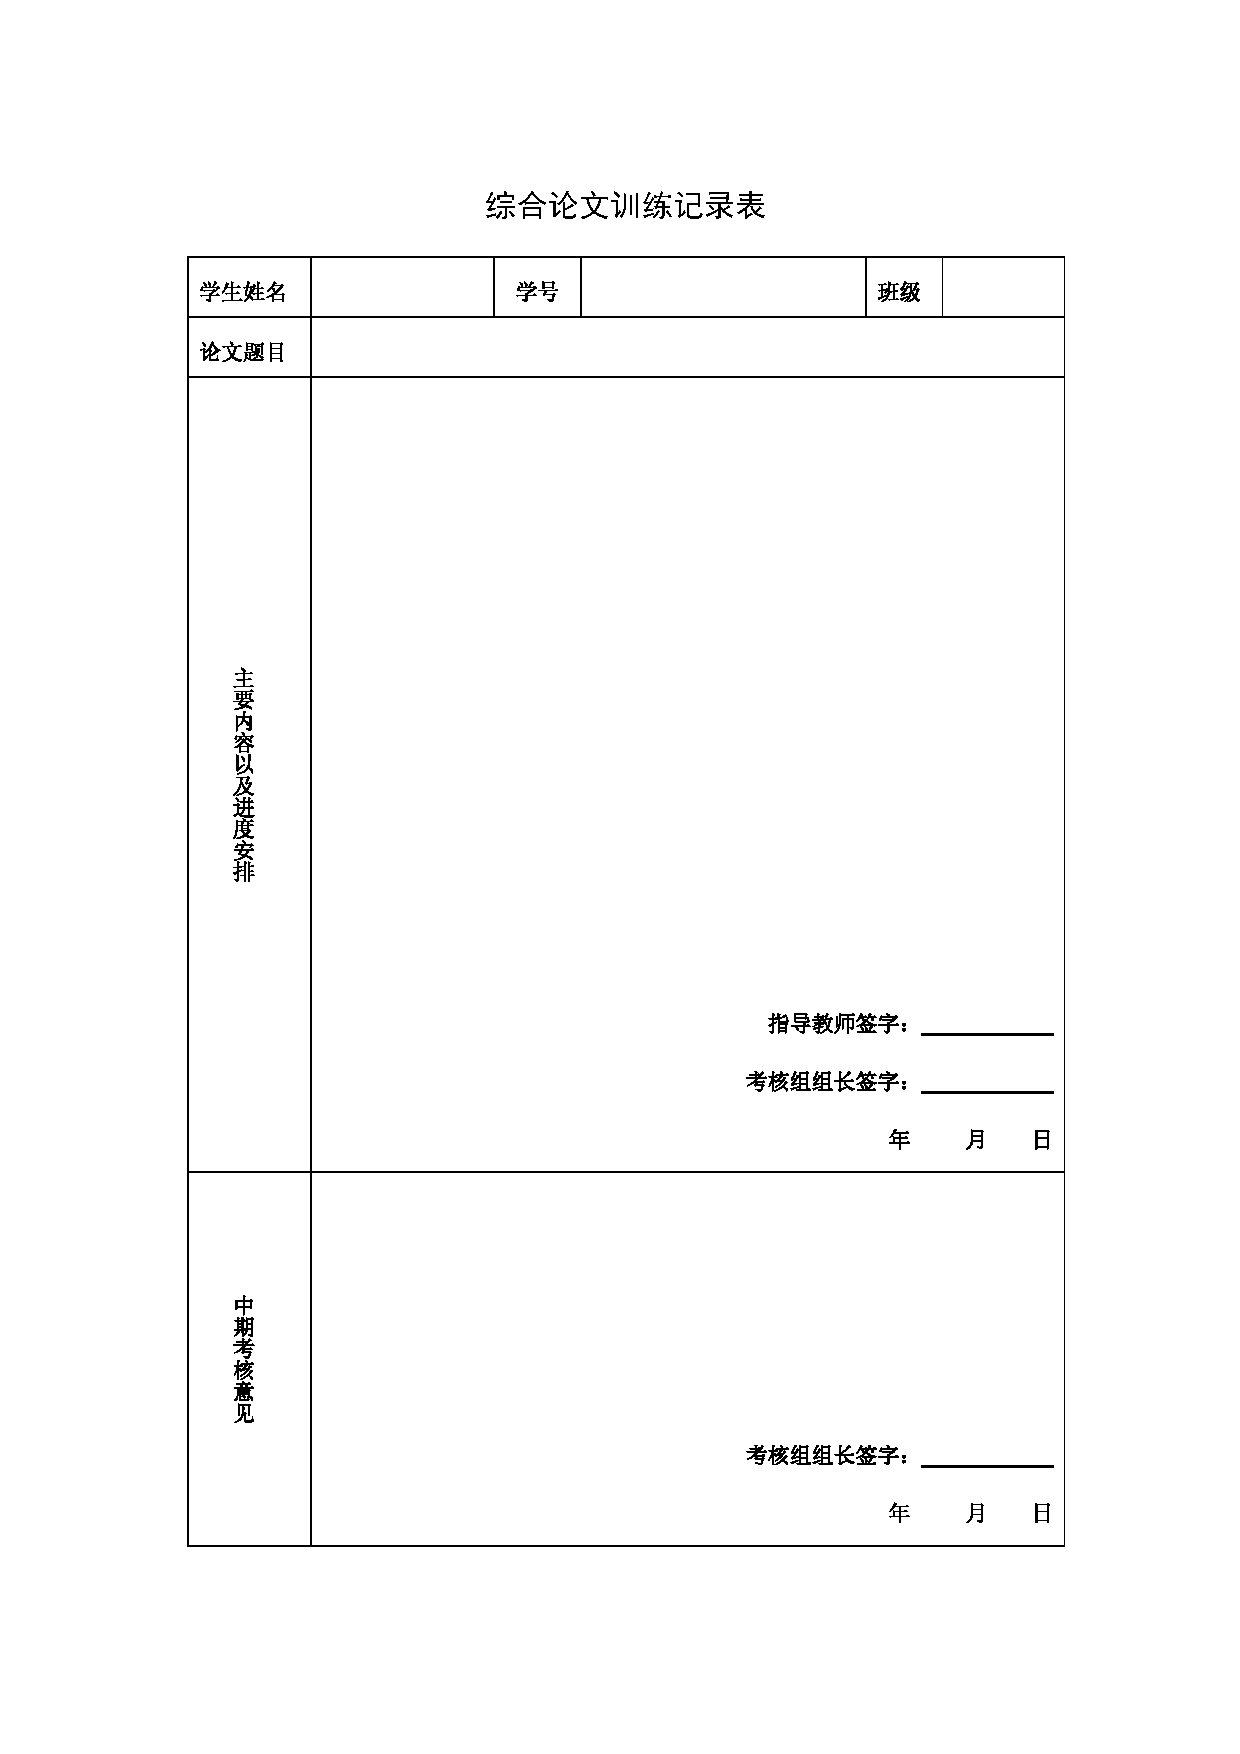
\includepdf[pages=-]{scan-record.pdf}
\end{document}
